% This file was created with tikzplotlib v0.10.1.
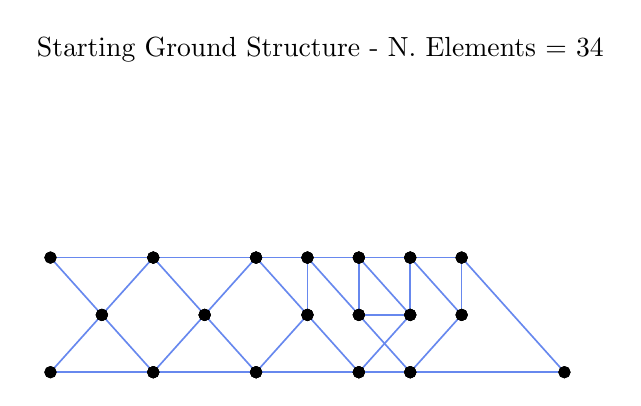
\begin{tikzpicture}

\definecolor{cornflowerblue103136238}{RGB}{103,136,238}
\definecolor{darkgray176}{RGB}{176,176,176}

\begin{axis}[
hide x axis,
hide y axis,
tick align=outside,
tick pos=left,
title={Starting Ground Structure - N. Elements = 34},
x grid style={darkgray176},
xmin=0, xmax=10.5,
xtick style={color=black},
y grid style={darkgray176},
ymin=-2.86209677419355, ymax=4.96209677419355,
ytick style={color=black}
]
\path [draw=cornflowerblue103136238, semithick]
(axis cs:0,0)
--(axis cs:1,1);

\path [draw=cornflowerblue103136238, semithick]
(axis cs:2,0)
--(axis cs:1,1);

\path [draw=cornflowerblue103136238, semithick]
(axis cs:2,0)
--(axis cs:3,1);

\path [draw=cornflowerblue103136238, semithick]
(axis cs:4,0)
--(axis cs:3,1);

\path [draw=cornflowerblue103136238, semithick]
(axis cs:4,0)
--(axis cs:5,1);

\path [draw=cornflowerblue103136238, semithick]
(axis cs:6,0)
--(axis cs:7,1);

\path [draw=cornflowerblue103136238, semithick]
(axis cs:6,0)
--(axis cs:7,0);

\path [draw=cornflowerblue103136238, semithick]
(axis cs:6,0)
--(axis cs:5,1);

\path [draw=cornflowerblue103136238, semithick]
(axis cs:7,0)
--(axis cs:6,1);

\path [draw=cornflowerblue103136238, semithick]
(axis cs:7,0)
--(axis cs:8,1);

\path [draw=cornflowerblue103136238, semithick]
(axis cs:1,1)
--(axis cs:0,2);

\path [draw=cornflowerblue103136238, semithick]
(axis cs:1,1)
--(axis cs:2,2);

\path [draw=cornflowerblue103136238, semithick]
(axis cs:3,1)
--(axis cs:2,2);

\path [draw=cornflowerblue103136238, semithick]
(axis cs:3,1)
--(axis cs:4,2);

\path [draw=cornflowerblue103136238, semithick]
(axis cs:5,1)
--(axis cs:4,2);

\path [draw=cornflowerblue103136238, semithick]
(axis cs:5,1)
--(axis cs:5,2);

\path [draw=cornflowerblue103136238, semithick]
(axis cs:6,1)
--(axis cs:7,1);

\path [draw=cornflowerblue103136238, semithick]
(axis cs:6,1)
--(axis cs:5,2);

\path [draw=cornflowerblue103136238, semithick]
(axis cs:6,1)
--(axis cs:6,2);

\path [draw=cornflowerblue103136238, semithick]
(axis cs:7,1)
--(axis cs:6,2);

\path [draw=cornflowerblue103136238, semithick]
(axis cs:7,1)
--(axis cs:7,2);

\path [draw=cornflowerblue103136238, semithick]
(axis cs:8,1)
--(axis cs:7,2);

\path [draw=cornflowerblue103136238, semithick]
(axis cs:8,1)
--(axis cs:8,2);

\path [draw=cornflowerblue103136238, semithick]
(axis cs:4,2)
--(axis cs:5,2);

\path [draw=cornflowerblue103136238, semithick]
(axis cs:5,2)
--(axis cs:6,2);

\path [draw=cornflowerblue103136238, semithick]
(axis cs:6,2)
--(axis cs:7,2);

\path [draw=cornflowerblue103136238, semithick]
(axis cs:7,2)
--(axis cs:8,2);

\path [draw=cornflowerblue103136238, semithick]
(axis cs:0,0)
--(axis cs:2,0);

\path [draw=cornflowerblue103136238, semithick]
(axis cs:2,0)
--(axis cs:4,0);

\path [draw=cornflowerblue103136238, semithick]
(axis cs:4,0)
--(axis cs:6,0);

\path [draw=cornflowerblue103136238, semithick]
(axis cs:10,0)
--(axis cs:7,0);

\path [draw=cornflowerblue103136238, semithick]
(axis cs:10,0)
--(axis cs:8,2);

\path [draw=cornflowerblue103136238, semithick]
(axis cs:0,2)
--(axis cs:2,2);

\path [draw=cornflowerblue103136238, semithick]
(axis cs:2,2)
--(axis cs:4,2);

\addplot [fill=black, mark=*, only marks]
table{%
x  y
0 0
1 1
};
\addplot [fill=black, mark=*, only marks]
table{%
x  y
2 0
1 1
};
\addplot [fill=black, mark=*, only marks]
table{%
x  y
2 0
3 1
};
\addplot [fill=black, mark=*, only marks]
table{%
x  y
4 0
3 1
};
\addplot [fill=black, mark=*, only marks]
table{%
x  y
4 0
5 1
};
\addplot [fill=black, mark=*, only marks]
table{%
x  y
6 0
7 1
};
\addplot [fill=black, mark=*, only marks]
table{%
x  y
6 0
7 0
};
\addplot [fill=black, mark=*, only marks]
table{%
x  y
6 0
5 1
};
\addplot [fill=black, mark=*, only marks]
table{%
x  y
7 0
6 1
};
\addplot [fill=black, mark=*, only marks]
table{%
x  y
7 0
8 1
};
\addplot [fill=black, mark=*, only marks]
table{%
x  y
1 1
0 2
};
\addplot [fill=black, mark=*, only marks]
table{%
x  y
1 1
2 2
};
\addplot [fill=black, mark=*, only marks]
table{%
x  y
3 1
2 2
};
\addplot [fill=black, mark=*, only marks]
table{%
x  y
3 1
4 2
};
\addplot [fill=black, mark=*, only marks]
table{%
x  y
5 1
4 2
};
\addplot [fill=black, mark=*, only marks]
table{%
x  y
5 1
5 2
};
\addplot [fill=black, mark=*, only marks]
table{%
x  y
6 1
7 1
};
\addplot [fill=black, mark=*, only marks]
table{%
x  y
6 1
5 2
};
\addplot [fill=black, mark=*, only marks]
table{%
x  y
6 1
6 2
};
\addplot [fill=black, mark=*, only marks]
table{%
x  y
7 1
6 2
};
\addplot [fill=black, mark=*, only marks]
table{%
x  y
7 1
7 2
};
\addplot [fill=black, mark=*, only marks]
table{%
x  y
8 1
7 2
};
\addplot [fill=black, mark=*, only marks]
table{%
x  y
8 1
8 2
};
\addplot [fill=black, mark=*, only marks]
table{%
x  y
4 2
5 2
};
\addplot [fill=black, mark=*, only marks]
table{%
x  y
5 2
6 2
};
\addplot [fill=black, mark=*, only marks]
table{%
x  y
6 2
7 2
};
\addplot [fill=black, mark=*, only marks]
table{%
x  y
7 2
8 2
};
\addplot [fill=black, mark=*, only marks]
table{%
x  y
0 0
2 0
};
\addplot [fill=black, mark=*, only marks]
table{%
x  y
2 0
4 0
};
\addplot [fill=black, mark=*, only marks]
table{%
x  y
4 0
6 0
};
\addplot [fill=black, mark=*, only marks]
table{%
x  y
10 0
7 0
};
\addplot [fill=black, mark=*, only marks]
table{%
x  y
10 0
8 2
};
\addplot [fill=black, mark=*, only marks]
table{%
x  y
0 2
2 2
};
\addplot [fill=black, mark=*, only marks]
table{%
x  y
2 2
4 2
};
\end{axis}

\end{tikzpicture}
